\documentclass[12pt]{article}

% --- Core Math & Physics Packages ---
\usepackage{amsmath, amssymb, amsthm, mathtools}
\usepackage{bm}          % Bold vectors (\vec{v})
\usepackage{esint}       % Multiple/surface integrals (\iint, \oiint)
\usepackage[margin=1in]{geometry}
\usepackage{parskip}     % Clean paragraph spacing without using '\\'
\usepackage[b]{esvect}
\usepackage{setspace}

% --- Formatting & Colored Boxes ---
\usepackage[most]{tcolorbox}
\usepackage{xcolor}

% --- Graphics & TikZ / 3D Plotting ---
\usepackage{tikz}
\usepackage{pgfplots}
\pgfplotsset{compat=1.18}
\usetikzlibrary{arrows.meta, calc}

% --- Custom Multivariable Macros ---
\newcommand{\pdv}[2]{\frac{\partial #1}{\partial #2}}
\newcommand{\grad}{\nabla}
\newcommand{\divg}{\nabla \cdot}
\newcommand{\curl}{\nabla \times}
\newcommand{\norm}[1]{\left\lVert #1 \right\rVert}
\newcommand{\ang}[1]{\left\langle #1 \right\rangle} % Angle brackets for vectors

% --- Custom Theorem Environments ---
\tcbuselibrary{theorems}

\newtcbtheorem[number within=section]{definition}{Definition}{
  colback=blue!5!white, 
  colframe=blue!60!black, 
  fonttitle=\bfseries
}{def}

\newtcbtheorem[number within=section]{problem}{Problem}{
  colback=orange!5!white, 
  colframe=orange!80!black, 
  fonttitle=\bfseries
}{prob}

\theoremstyle{definition}
\newtheorem{example}{Example}[section]

\setstretch{1.5}
% ------------------------------------------------------------------
\begin{document}

\section{Vectors in Two and Three Dimensions}

\paragraph{Question:} What information specifies a line?
\begin{itemize}
    \item 2 points
    \item A point and a direction vector
    \item Slope and $y$-intercept
    \item Intersection of 2 non-parallel planes
\end{itemize}

\paragraph{Comparison:}
\begin{itemize}
    \item \textbf{Single-variable calculus:} $f(x) \rightarrow \text{rate of change of } x$
    \item \textbf{Multivariable calculus:} $f(x,y) \rightarrow \text{functions of multiple variables}$
\end{itemize}

% ------------------------------------------------------------------

\subsection{Coordinates}

\begin{center}
% --- 2D Section ---
\begin{minipage}[t]{0.48\textwidth}
    \textbf{2-dimension (2D):} $(2,3)$
    \vspace{0.5em}

    \centering
    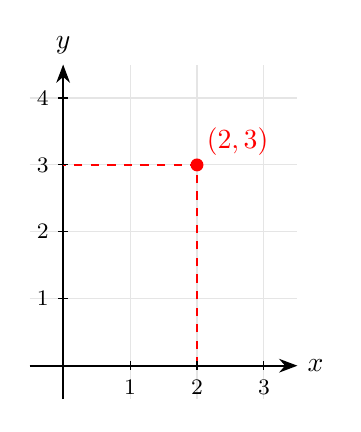
\begin{tikzpicture}[scale=0.85, >=Stealth]
        % Grid and axes
        \draw[thin, gray!20] (-0.5,-0.5) grid (3.5,4.5);
        \draw[->, thick] (-0.5,0) -- (3.5,0) node[right] {$x$};
        \draw[->, thick] (0,-0.5) -- (0,4.5) node[above] {$y$};
        
        % Dashed Projection Lines
        \draw[dashed, red, thick] (2,0) -- (2,3) -- (0,3);
        
        % Point Plot
        \filldraw[red] (2,3) circle (2.5pt) node[above right] {$(2,3)$};
        
        % Axis ticks
        \foreach \x in {1,2,3}
            \draw (\x,2pt) -- (\x,-2pt) node[below] {\footnotesize $\x$};
        \foreach \y in {1,2,3,4}
            \draw (2pt,\y) -- (-2pt,\y) node[left] {\footnotesize $\y$};
    \end{tikzpicture}
\end{minipage}
\hfill
% --- 3D Section ---
\begin{minipage}[t]{0.48\textwidth}
    \textbf{3-dimension (3D):} $(1, \pi, 3)$
    \vspace{0.5em}

    \centering
    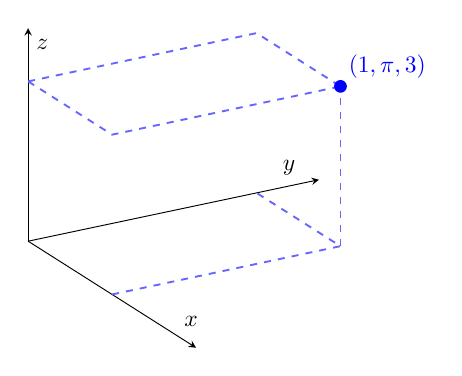
\begin{tikzpicture}[scale=0.85]
    \begin{axis}[
        view={60}{30},
        axis lines=center,
        xlabel={$x$}, ylabel={$y$}, zlabel={$z$},
        xmin=0, xmax=2,
        ymin=0, ymax=4,
        zmin=0, zmax=4,
        ticks=none,
        enlargelimits=false
    ]
        % Coordinates: x=1, y=pi (~3.14), z=3
        % Projection box (dashed lines)
        \draw[dashed, blue!60, thick] (axis cs:1,0,0) -- (axis cs:1,3.14159,0) -- (axis cs:0,3.14159,0);
        \draw[dashed, blue!60, thick] (axis cs:1,3.14159,0) -- (axis cs:1,3.14159,3);
        \draw[dashed, blue!60, thick] (axis cs:0,0,3) -- (axis cs:1,0,3) -- (axis cs:1,3.14159,3);
        \draw[dashed, blue!60, thick] (axis cs:0,0,3) -- (axis cs:0,3.14159,3) -- (axis cs:1,3.14159,3);

        % Point Plot
        \addplot3[only marks, mark=*, mark size=2.5pt, color=blue] 
            coordinates {(1, 3.14159, 3)};
        
        % Node Label
        \node[above right, color=blue] at (axis cs:1, 3.14159, 3) {$(1, \pi, 3)$};
    \end{axis}
    \end{tikzpicture}
\end{minipage}
\end{center}

% ------------------------------------------------------------------
\subsection{Vectors and Position Vectors}

Given points $P=(1,3)$, $Q=(5,4)$ and $P'=(1,1)$, $Q'=(5,2)$:

\begin{definition}{Equivalent Vectors}{equiv_vectors}
Two vectors are \textbf{equivalent} if one is a translation (pure shift without rotation) of the other.
\end{definition}

\begin{example}
Let $R = (4,1)$ and $O = (0,0)$. Then:
\[
\vv{PQ} = \vv{P'Q'} = \vv{OR}
\]
\end{example}

\begin{definition}{Position Vector}{pos_vector}
A vector whose initial point is at the origin $O(0,0)$ is called a \textbf{position vector}. It is written using angle brackets:
\[
\vv{OR} = \ang{4, 1}
\]
\end{definition}

\begin{definition}{Magnitude / Norm}{magnitude}
The \textbf{length} or \textbf{magnitude} of a vector $\vv{v}$, denoted by $\norm{\vv{v}}$, is the length of the line segment between its endpoints.
\end{definition}

If $\vv{v} = \ang{v_1, v_2}$, then its magnitude is given by:
\[
\norm{\vv{v}} = \sqrt{v_1^2 + v_2^2}
\]

For example, using $\vv{PQ} = \ang{4,1}$:
\[
\norm{\vv{PQ}} = \sqrt{4^2 + 1^2} = \sqrt{17}
\]

% ------------------------------------------------------------------
\subsection{Unit Vectors}

A vector $\vv{v}$ is called a \textbf{unit vector} if its magnitude is 1, i.e., $\norm{\vv{v}} = 1$.

\begin{problem}{Describing Unit Vectors}{unit_vectors}
Describe all unit vectors in $\mathbb{R}^2$.

A vector $\vv{v} = \ang{x, y}$ is a unit vector if and only if $x^2 + y^2 = 1$. Equivalently, using polar parameterization:
\[
\vv{v}(t) = \ang{\cos t, \sin t} \quad \text{for } 0 \le t < 2\pi
\]

% --- Unit Circle TikZ Plot ---
\begin{center}
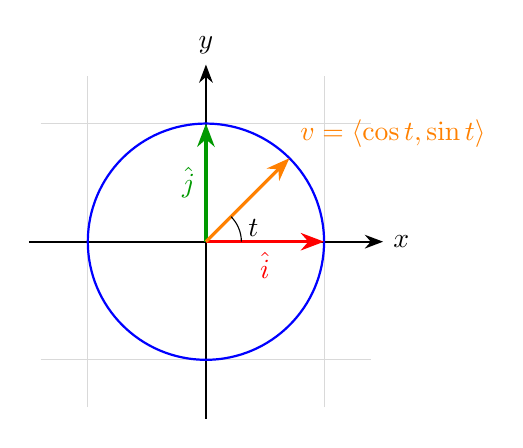
\begin{tikzpicture}[scale=1.5, >=Stealth]
    % Grid and axes
    \draw[thin, gray!30] (-1.4,-1.4) grid (1.4,1.4);
    \draw[->, thick] (-1.5,0) -- (1.5,0) node[right] {$x$};
    \draw[->, thick] (0,-1.5) -- (0,1.5) node[above] {$y$};
    
    % Unit circle
    \draw[blue, thick] (0,0) circle (1cm);
    
    % Standard basis vectors
    \draw[->, very thick, red] (0,0) -- (1,0) node[midway, below] {$\hat{i}$};
    \draw[->, very thick, green!60!black] (0,0) -- (0,1) node[midway, left] {$\hat{j}$};
    
    % Arbitrary unit vector
    \draw[->, very thick, orange] (0,0) -- (45:1cm) node[above right] {$\vv{v} = \ang{\cos t, \sin t}$};
    \draw (0.3,0) arc (0:45:0.3cm) node[midway, right] {$t$};
\end{tikzpicture}
\end{center}

\end{problem}

\paragraph{Standard Basis Vectors:}
\begin{itemize}
    \item \textbf{2D Basis Vectors:} $\hat{i} = \ang{1,0}$, \quad $\hat{j} = \ang{0,1}$
    \item \textbf{3D Basis Vectors:} $\hat{i} = \ang{1,0,0}$, \quad $\hat{j} = \ang{0,1,0}$, \quad $\hat{k} = \ang{0,0,1}$
\end{itemize}

% ------------------------------------------------------------------
\subsection{Vector Operations}

\paragraph{Addition and Subtraction:}
\begin{align*}
    \ang{v_1, v_2} + \ang{w_1, w_2} &= \ang{v_1 + w_1, v_2 + w_2} \\
    \ang{v_1, v_2} - \ang{w_1, w_2} &= \ang{v_1 - w_1, v_2 - w_2} \quad \text{(Equivalent to } \vv{v} + (-1)\vv{w}\text{)}
\end{align*}

\paragraph{Scalar Multiplication:}
For any scalar $\lambda \in \mathbb{R}$ and vector $\vv{v} = \ang{v_1, v_2}$:
\[
\lambda \vv{v} = \ang{\lambda v_1, \lambda v_2}
\]

% --- Parallelogram Rule TikZ Plot ---
\begin{center}
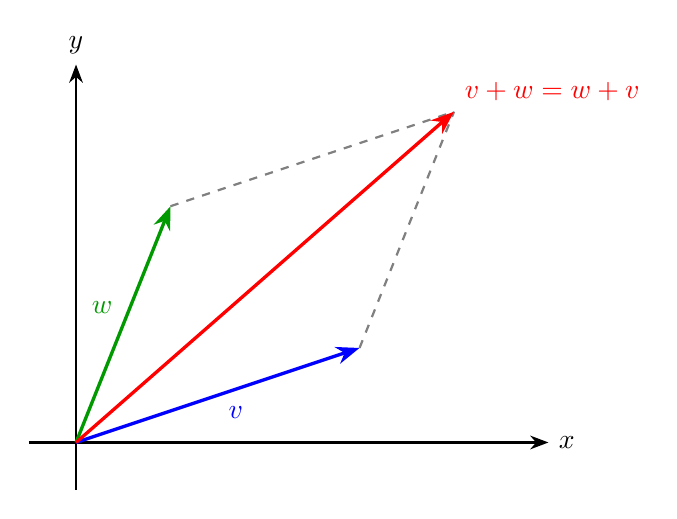
\begin{tikzpicture}[scale=1.2, >=Stealth]
    \draw[->, thick] (-0.5,0) -- (5,0) node[right] {$x$};
    \draw[->, thick] (0,-0.5) -- (0,4) node[above] {$y$};
    
    % Vectors
    \coordinate (O) at (0,0);
    \coordinate (V) at (3,1);
    \coordinate (W) at (1,2.5);
    \coordinate (VW) at (4,3.5);
    
    \draw[->, very thick, blue] (O) -- (V) node[midway, below right] {$\vv{v}$};
    \draw[->, very thick, green!60!black] (O) -- (W) node[midway, above left] {$\vv{w}$};
    
    % Dashed parallelogram lines
    \draw[dashed, thick, gray] (V) -- (VW);
    \draw[dashed, thick, gray] (W) -- (VW);
    
    % Resultant vector
    \draw[->, very thick, red] (O) -- (VW) node[above right] {$\vv{v} + \vv{w} = \vv{w} + \vv{v}$};
\end{tikzpicture}
\end{center}

\begin{tcolorbox}[colback=red!5!white, colframe=red!75!black, title=Important Note]
Vectors are \textbf{not} designed to be divided! (Vector division is undefined).
\end{tcolorbox}



% ------------------------------------------------------------------
\subsection{Parallel Vectors}

\begin{definition}{Parallel Vectors}{parallel_vectors}
Two non-zero vectors $\vv{v}$ and $\vv{w}$ ($\vv{v}, \vv{w} \neq \ang{0,0}$) are \textit{parallel} (denoted as $\vv{v} \parallel \vv{w}$) if there exists a non-zero scalar $\lambda \in \mathbb{R}$ such that:
\[
\vv{w} = \lambda \vv{v}
\]
\end{definition}

\paragraph{Equivalent Geometric Definition:}
$\vv{v} \parallel \vv{w}$ if and only if both vectors define or lie on the \textit{same line passing through the origin.}

\section{Discussion Week 1: Distance Formulae and Geometric Shapes}

\begin{definition}{Distance Formula in $\mathbb{R}^2$}{dist_2d}
Let $(x,y) \in \mathbb{R}^2$ and points $P=(x_1,y_1)$, $Q=(x_2,y_2)$. The distance between $P$ and $Q$ is given by:
\[
d(P,Q) = \norm{\vec{PQ}} = \sqrt{(x_2-x_1)^2 + (y_2-y_1)^2}
\]
\end{definition}

This distance formula is a direct application of the Pythagorean theorem, where the distance $d(P,Q)$ forms the hypotenuse of a right-angled triangle with legs $|x_2 - x_1|$ and $|y_2 - y_1|$.

\begin{figure}[htbp]
\centering
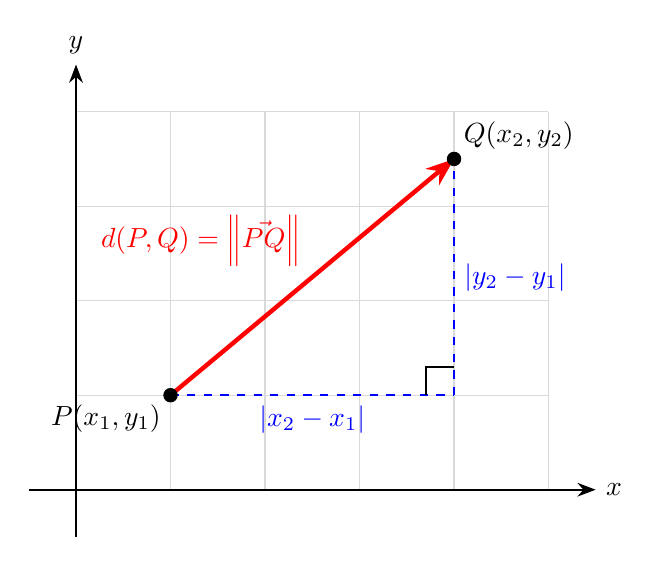
\begin{tikzpicture}[scale=1.2]
    % Grid and axes
    \draw[thin, gray!30] (0,0) grid (5,4);
    \draw[-{Stealth}, thick] (-0.5,0) -- (5.5,0) node[right] {$x$};
    \draw[-{Stealth}, thick] (0,-0.5) -- (0,4.5) node[above] {$y$};
    
    % Points
    \coordinate (P) at (1,1);
    \coordinate (Q) at (4,3.5);
    \coordinate (R) at (4,1);
    
    % Triangle legs
    \draw[dashed, blue, thick] (P) -- (R) node[midway, below] {$|x_2 - x_1|$};
    \draw[dashed, blue, thick] (R) -- (Q) node[midway, right] {$|y_2 - y_1|$};
    
    % Hypotenuse / Vector
    \draw[-{Stealth}, red, ultra thick] (P) -- (Q) node[midway, above left] {$d(P,Q) = \norm{\vec{PQ}}$};
    
    % Draw right angle symbol
    \draw[thick] (3.7,1) -- (3.7,1.3) -- (4,1.3);
    
    % Label Points
    \filldraw (P) circle (2pt) node[below left] {$P(x_1,y_1)$};
    \filldraw (Q) circle (2pt) node[above right] {$Q(x_2,y_2)$};
\end{tikzpicture}
\caption{Vector $\vec{PQ}$ in $\mathbb{R}^2$ visualized using the Pythagorean theorem.}
\end{figure}

The case in $\mathbb{R}^3$ follows similarly:

\begin{definition}{Distance Formula in $\mathbb{R}^3$}{dist_3d}
Let $(x,y,z) \in \mathbb{R}^3$ and points $P=(x_1,y_1,z_1)$, $Q=(x_2,y_2,z_2)$. The distance between $P$ and $Q$ is given by:
\[
d(P,Q) = \norm{\vec{PQ}} = \sqrt{(x_2-x_1)^2 + (y_2-y_1)^2 + (z_2-z_1)^2}
\]
\end{definition}

\subsection{Equations of Geometric Shapes}

Consider the equation $x^2 + y^2 = 4$.

In $\mathbb{R}^2$, this equation is equivalent to the set:
\[
\{(x,y) \in \mathbb{R}^2 : x^2 + y^2 = 4\}
\]
This represents a circle with radius $r=2$ centered at the origin. The distance from the origin $(0,0)$ to any point $(x,y)$ on this circle is constant and equal to 2, which can be verified directly using the distance formula:
\[
\sqrt{(x-0)^2 + (y-0)^2} = 2
\]
Hence, the geometry of the circle is directly implied by the Pythagorean theorem.

Now consider the equation $x^2 + y^2 = 1$ in three-dimensional space, $\mathbb{R}^3$. This set is formally expressed as:
\[
\{(x,y,z) \in \mathbb{R}^3 : x^2 + y^2 = 1\}
\]
Because $z$ is completely unrestricted, the cross-section at any constant height $z=c$ forms the unit circle $x^2 + y^2 = 1$. Consequently, this equation describes a \textit{right circular cylinder} extending infinitely along the $z$-axis.

\begin{figure}[htbp]
\centering
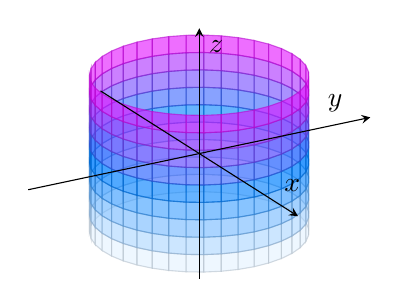
\begin{tikzpicture}
\begin{axis}[
    axis lines=center,
    axis on top,
    xlabel={$x$},
    ylabel={$y$},
    zlabel={$z$},
    xmin=-1.5, xmax=1.5,
    ymin=-1.5, ymax=1.5,
    zmin=-2, zmax=2,
    ticks=none,
    enlargelimits=true,
    view={60}{30}
]
    % Cylinder plot
    \addplot3[
        surf,
        domain=0:360,
        domain y=-1.5:1.5,
        samples=40,
        samples y=10,
        variable=\t,
        variable y=\z,
        colormap/cool,
        opacity=0.6
    ]
    ({cos(t)}, {sin(t)}, {\z});
    
\end{axis}
\end{tikzpicture}
\caption{The equation $x^2 + y^2 = 1$ plotted in $\mathbb{R}^3$ forms a right circular cylinder.}
\end{figure}

\subsection{Linear Equations across Dimensions}

In $\mathbb{R}^2$, the general form of a linear equation is given by:
\[
Ax + By + C = 0 \quad (A, B, C \in \mathbb{R}, \text{ with } A \text{ and } B \text{ not both zero})
\]
This equation represents a \textit{line} in two-dimensional space.

In $\mathbb{R}^3$, however, the exact same algebraic equation $Ax + By + C = 0$ represents a \textit{plane} parallel to the $z$-axis (since $z$ is a free variable), not a line. 

To uniquely define a line in three-dimensional space, a single linear equation is insufficient; we require a system of \textit{two} independent linear equations (representing the intersection of two non-parallel planes).

\end{document}